% Source of "When the Harness Answers 'A'". Every number in this file is re-derived from
% outputs/*.json by scripts/check_paper_numbers.py, which fails the build on disagreement.
\documentclass{article}

\usepackage[final]{nejlt}
%\usepackage[final]{nejlt}

\usepackage{booktabs}
\usepackage{graphicx}
\usepackage{amsmath}
\usepackage[T1]{fontenc}
\usepackage[utf8]{inputenc}
\usepackage{url}
\Urlmuskip=0mu\relax
\def\UrlBreaks{\do\/\do\-\do\_\do\.\do\:}
\emergencystretch=2em

\title{When the Harness Answers ``A'': Score-Inflating Evaluation Bugs Camouflaged by Model Bias}

\makeatletter
\edef\headtitle{When the Harness Answers ``A''}%
\makeatother

\author{
Taleef Tamsal, Purdue University Fort Wayne, Indiana, USA {\tt \small tamst01@pfw.edu} \and
Jonathan Rusert, Purdue University Fort Wayne, Indiana, USA {\tt \small jrusert@pfw.edu}
}

\begin{document}
\thispagestyle{title}

\abstract{Evaluation harnesses are usually studied as a source of \emph{variance}: format sensitivity, extraction choices, and implementation drift that move scores unpredictably. We document a more dangerous class of harness fault: bugs that reliably \emph{inflate} accuracy, so a leaderboard cannot see them, and that are \emph{camouflaged} because their symptom coincides with a documented model behaviour. Auditing a multiple-choice document-QA pipeline that ranked mid-field in a shared task, we find two such bugs: a stop sequence that halts generation at token zero, so the empty output is parsed as a fixed ``A'', and a prefix-cache reuse in a widely-used local-inference binding that collapses three-pass self-consistency voting into a single decision. Both \emph{raise} the reported score, and both hide behind option-``A'' bias, a documented property of multiple-choice language models, so the literature that names the symptom is what suppresses debugging. We then show that the same camouflage converts ordinary tool defaults into apparent \emph{language}, \emph{modality}, and \emph{quantization} failures across three controlled experiments, we report two language-shaped hypotheses of our own that instrumentation refuted, and we verify that the underlying bug classes recur in widely-used public tooling. We close with an auditing checklist. No model and no language is the weak link here. A wrong number that looks reasonable is indistinguishable from a right one until you instrument the path that produced it.}

\maketitle

\section{Introduction}

Most work on evaluation reliability treats the harness as a source of noise: change the prompt format and rankings move \cite{sclar2024formatspread}; change the implementation and benchmark scores shift \cite{alzahrani2024benchmarks}; leave harness details implicit and results fail to reproduce \cite{biderman2024lessons}. This framing has a blind spot. It assumes the failure mode is a \emph{wrong-looking} number: one that varies, or disagrees across runs, and so invites scrutiny. The failures we report do the opposite: they produce a \emph{right-looking} number that is quietly too high.

Two properties make them hard to catch. First, \textbf{they inflate}. A leaderboard ranks the number and nothing else, so it cannot flag a fault that improves your standing; the incentive to investigate points the wrong way. Second, \textbf{they are camouflaged}: the visible symptom is a behaviour the literature already documents. In multiple-choice evaluation, language models are known to be biased toward the first option \cite{zheng2024selectors}. When a harness bug \emph{also} produces excess ``A''s, it wears that finding as a disguise. The explanation is already on the shelf, so no one debugs.

We observed this directly. \textbf{Every failure path in our pipeline terminates at the answer ``A''}: a parser that finds no letter returns ``A''; an empty generation is parsed as ``A''; a cache-corrupted vote resolves to ``A''. For a week we read each one as option-A bias.

The system in question is a retrieval-augmented multiple-choice pipeline for document question answering over Ukrainian PDFs, built for a shared task, where it placed mid-field. That setting matters to the argument in a specific way. In multilingual and low-resource evaluation, ``the language is hard'' is an always-available explanation, and it is the one we reached for. Before instrumenting anything we had written down two tidy, arithmetic accounts of why an English-tuned pipeline would break in Ukrainian. Both were false, and we report them as nulls. The failures were in the tools.

We make four contributions.

\textbf{(i)} We characterize \emph{score-inflating, camouflaged} harness bugs as a class, and give two worked instances in a real ranked system, including one (prefix-cache reuse corrupting self-consistency voting) that follows from a documented property of a widely-used local-LLM binding but is, to our knowledge, undocumented in its effect on voting.

\textbf{(ii)} We show the same camouflage drives \emph{misattribution}: three controlled experiments in which a tool default is read as a fact about a language, a modality, or a quantization setting, and a matched control localizes each to the tool.

\textbf{(iii)} We report two language-shaped hypotheses of our own that instrumentation refuted, and one claim we made, pre-registered, and were forced to retract. Together they are evidence that the camouflage is not a failure of other people's diligence.

\textbf{(iv)} We verify the three bug classes in public, widely-used tooling, and distill an auditing checklist.

Throughout, every quantitative claim is re-derived from raw artifacts by a checker that fails the build on disagreement, and the audited pipeline, the audit artifacts, and the checker are released (Section~\ref{sec:availability}).

\section{Related Work}

Harness artifacts are known to move scores. Prompt formatting alone changes rankings \cite{sclar2024formatspread}; benchmark scores are unstable across implementation choices \cite{alzahrani2024benchmarks}; reproducible evaluation requires pinning normally-implicit harness details \cite{biderman2024lessons}. Answer extraction is a documented culprit in particular: \newcite{molfese2025rightanswer} show that the \emph{same} model outputs receive different accuracy under different extraction methods, and construct an adversarial benchmark to expose it. The nondeterminism behind our second bug is a documented property of batched inference \cite{he2025nondeterminism}, and is acknowledged in the inference engine we use \cite{llamacpp}.

We extend this literature in three ways.

\textbf{Direction.} Prior work studies variance, and the faults it documents are mostly score-\emph{deflating} or rank-\emph{reordering}: the number looks wrong, or moves when it should not, which is what invites investigation. The faults we document \emph{inflate} accuracy. They are invisible to a leaderboard by construction, and the party best positioned to find them is the party whose score benefits.

\textbf{Camouflage.} A harness bug can be masked by a documented \emph{model} behaviour. Option-A bias \cite{zheng2024selectors} is a real and well-replicated finding; it is also a ready-made explanation for a symptom that a parser bug produces. The literature that names the symptom actively suppresses the debugging. We are not aware of this mechanism being named previously, and we think it generalizes past our case: any harness fault whose signature coincides with a known model pathology inherits that pathology's explanatory cover.

\textbf{Misattribution.} We give three cases in which a tool default is mistaken for a property of a language, a modality, or a quantization setting. This matters especially in multilingual and low-resource evaluation, where a typological explanation is always available and rarely challenged, and where the tooling is most likely to carry defaults tuned on English.

\section{The Audited System}
\label{sec:system}

We audit a retrieval-augmented multiple-choice pipeline for document question answering over Ukrainian PDFs \cite{unlp2026task}. Given a question with six options, the system predicts an answer letter, a source document, and a page within that document. The official score is
\[
0.5\,\bar a + 0.25\,\bar d + 0.25\,\bar p,
\]
where $\bar a$ and $\bar d$ are mean answer- and document-correctness and page proximity is
\[
p_i = 1 - \frac{|\mathrm{Page}^{\mathrm{pred}}_i - \mathrm{Page}^{\mathrm{true}}_i|}{n_i}
\]
when the document is correct and $0$ otherwise, with $n_i$ the true page count of the gold document. We verified this implementation against the official definition.

The pipeline retrieves with BGE-M3 dense embeddings \cite{chen2024bgem3}, reranks candidate pages with a Qwen3 cross-encoder \cite{qwen3_2025}, and answers with a 4-bit Ukrainian-adapted Gemma-3-12B \cite{mamaylm2025} served through \texttt{llama.cpp} \cite{llamacpp}, using three-pass self-consistency voting. It ran under a fixed offline compute budget, which is why the answering model is quantized and the generation budget is small. Both turn out to matter.

All analyses below are over a 461-question development set and are reproducible from committed artifacts. The submitted source is part of the released repository (Section~\ref{sec:availability}). The audited run voted stochastically; to separate harness behaviour from sampler behaviour, the determinism analyses in Section~\ref{sec:cache} use a reconstruction with the vote temperature set to zero, which isolates the cache effect. We do not equate any number here with the private-test leaderboard score.

\section{Two Score-Inflating Harness Bugs}
\label{sec:bugs}

\begin{figure}[t]
\centering
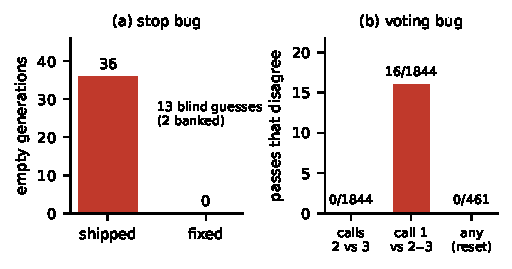
\includegraphics[width=\columnwidth]{fig_bugs.pdf}
\caption{Both bugs leave a checkable footprint on the reconstruction; every count in the panels is read
from the raw logs rather than typed. \textbf{(a)} The stop sequence empties a block of generation calls
as shipped and none once fixed, and those empty strings become blind ``A'' guesses, two of which are
banked as correct. \textbf{(b)} At vote temperature zero the two cache-warmed passes never disagree
while the first pass sometimes does; forcing a true reset makes every pass identical.}
\label{fig:bugs}
\end{figure}

\subsection{A Stop Sequence That Empties the Generation}
\label{sec:stop}

The answering prompt ends with a colon and no trailing space, so the model's natural continuation begins with a newline. The character \verb|"\n"| was in the stop list. Generation therefore halted at \textbf{token zero} and returned the empty string.

The failure is invisible to the obvious guard. The completion carries \verb|finish_reason="stop"|, never \verb|"length"|, because the generation did not run out of budget but was stopped on the first token, so a truncation check cannot catch it. The answer parser then falls through every branch to an unconditional \verb|return "A"|.

On \textbf{36 of 1,383} generation calls the pipeline received nothing and answered ``A'' (Figure~\ref{fig:bugs}a). Those empty strings decided \textbf{13 questions} by a blind guess, of which \textbf{2} were correct by chance and banked as knowledge. Reported answer accuracy was 0.8807; had the guesses abstained it would have been 0.8764, so the bug manufactured \textbf{0.43} points of answer accuracy.

It stayed invisible because three things hid it simultaneously: the model appeared to answer, ``A'' is a plausible answer, and language models are already documented to favour option A \cite{zheng2024selectors}. A parser failure wore the costume of a model behaviour.

\subsection{Two Language-Shaped Hypotheses, Both Null}
\label{sec:nulls}

Before instrumenting anything, we had an account of this failure that named the language as the cause, and it was arithmetic. Our answering stage capped generation at three tokens. The string \emph{``Answer: A''} is exactly three tokens in English; its Ukrainian equivalent is five under the answering model's vocabulary. A budget adequate in English is arithmetically insufficient in Ukrainian. We had a second such story: the model would emit Cyrillic homoglyphs where our parser looked for Latin letters, and the mismatch would silently drop answers.

Both are false. We report them as nulls, and we regard reporting them as the paper's method rather than as a limitation: the language-shaped explanation was available, plausible, on-thesis, and wrong, and only instrumentation told us so.

\textbf{The budget never binds.} In the shipped configuration, the number of truncated calls is \textbf{zero}. The budget cannot bind if nothing is ever truncated, because the stop sequence fires first. Raising the budget from 3 to 8 changed nothing: the resulting run is byte-identical to the original. The null is vacuous by construction, and we say so rather than reporting ``no significant effect of budget''.

\textbf{The budget does not bind even after the fix.} With the newline stop removed, six parser fallbacks remain, and all of them finish with \verb|reason="length"|, so the natural reading is that the model began quoting the document and ran out of room. That reading is also wrong, and we tested it rather than assuming it. At a budget of 64, truncation falls from 6 to 0 while the fallback count stays at 6. Given eight times the room, the model finishes its sentence and still never emits a letter: it answers by quoting the document in Ukrainian prose. The budget was never the binding constraint, not at 3, not at 8, not at 64.

\textbf{The homoglyph failure does not occur.} The extractor's Cyrillic-prefix branch is instrumented, and it fires \textbf{0 times in 5,532 calls} across all four experimental cells. The hypothesis is dead.

Table~\ref{tab:cells} gives the instrumented counts. Removing the newline from the stop list drives empty generations from 36 to 0, parser fallbacks from 36 to 6, and questions decided by a blind ``A'' from 13 to 2.

\begin{table*}
\centering
\begin{tabular}{llrrrr}
\toprule
\textbf{cell} & \textbf{configuration} & \textbf{empty} & \textbf{truncated} & \textbf{fallback} & \textbf{Cyrillic} \\
\midrule
\texttt{e2e\_b3}    & budget 3, stop \verb|[\n, .]| (as shipped)    & 36 & 0 & 36 & 0 \\
\texttt{e2e\_b8}    & budget 8, stop \verb|[\n, .]| (budget hypothesis) & 36 & 0 & 36 & 0 \\
\texttt{e2e\_fix}   & budget 8, stop \verb|[.]| (the fix)           & 0  & 6 & 6  & 0 \\
\texttt{e2e\_fix64} & budget 64, stop \verb|[.]| (budget $\times 8$) & 0  & 0 & 6  & 0 \\
\bottomrule
\end{tabular}
\caption{Instrumented answer-path counts across the four cells. The answer-budget hypothesis is a no-op both before the fix and after it; the homoglyph branch never fires.}
\label{tab:cells}
\end{table*}

\subsection{A Prefix Cache That Corrupts Self-Consistency Voting}
\label{sec:cache}

The pipeline casts three votes per question. With the vote temperature at zero, all three passes are greedy calls on a \textbf{byte-identical prompt}, and must return identical text. They do not.

The cause is in the inference binding, not in our code. Inside its generation loop, on a prefix-cache hit the library \textbf{cancels its own reset}: it detects that the incoming tokens share a prefix with what is already cached, sets the reset flag to false, truncates the input to the unshared suffix, and decodes that suffix on top of a warm KV cache. Because the scoring function calls the same prompt three times in a row, call~1 arrives with the \emph{previous question's} prompt cached and evaluates a long divergent suffix, while calls~2 and~3 find the whole prompt already cached and evaluate exactly one token.

That this changes the output, and not merely the speed, follows from a documented property of non-batch-invariant kernels. GPU kernels select a parallel reduction strategy from the shape of the work, and floating-point accumulation is not associative. \newcite{he2025nondeterminism} state our exact case: the reduction order must be identical regardless of whether zero tokens are in the KV cache during prefill or many are during decoding, and handling the cache separately from the current token values breaks batch invariance. Different cache length gives a different reduction order, hence different logits, hence a different greedy token, all from a byte-identical prompt.

Nor is this a property of GPUs imported from elsewhere. It is documented in the tool we ran: the \texttt{llama.cpp} server documentation warns, for its prompt-cache option, that logits are not guaranteed to be bit-for-bit identical across batch sizes and that this can cause nondeterministic results, and an issue on its tracker demonstrates the effect concretely \cite{llamacpp_issue4479}. What our pipeline hit is that acknowledged behaviour, reached silently: the Python binding reuses the prefix cache by default and surfaces no warning to the caller. It is also not a quirk of our pinned version. We read the reuse path both in the release we shipped and at the then-current HEAD; both still truncate a byte-identical prompt to its shared prefix and decode against a warm cache. The newer code adds a one-token logits refresh for the exact-cache-hit case, but does not remove the batch-size mismatch that drives the divergence. The hazard ships today.

The mechanism makes a \textbf{falsifiable prediction}. Calls~2 and~3 share one code path, so they must \emph{always} agree with each other, while call~1 may differ. That is what the traces show (Figure~\ref{fig:bugs}b). Across all cells:

\begin{itemize}
\itemsep=0pt
\item calls 2 vs.\ 3 disagree on \textbf{0 of 1,844} vote-triples;
\item call~1 differs from calls 2--3 on 4 of 461 questions.
\end{itemize}

Votes 2 and 3 are not independent samples. They are numerically identical twins. Forcing an explicit reset before every call makes all three passes return identical text on \textbf{461/461} questions, confirming the diagnosis; because the model handle is used only in the answering stage, document accuracy comes back bit-identical, which confirms the intervention was surgical.

A corollary: in a clean harness the three-pass vote is \emph{provably} a no-op. All three calls are identical, so it is mathematically incapable of changing any answer, at three times the inference cost.

\subsection{The Two Bugs Compound}

Majority voting lets calls~2 and~3 overrule call~1 only by agreeing with each other, which the warm cache guarantees they do. Add the stop-list bug: when calls~2 and~3 lead with a newline they return the empty string, both are parsed as ``A'', and \textbf{two empty strings outvote the model's answer, two to one}.

Every failure path in this harness leads to ``A''. An empty generation falls back to A; the warm-cache calls drift to A; two corrupted votes outvote one uncorrupted one. Option-A bias is real, and it is also perfect camouflage for bugs that share its signature.

\subsection{The Score Ladder, and Why It Is Not the Evidence}
\label{sec:ladder}

Table~\ref{tab:ladder} gives the three-rung ladder. \textbf{Correcting both bugs lowers the score.}

\begin{table*}
\centering
\begin{tabular}{lrrrrl}
\toprule
\textbf{system} & \textbf{correct} & \textbf{answer} & \textbf{composite} & \textbf{blind ``A''} & \\
\midrule
as shipped          & 406/461 & 0.880694 & 0.880780 & 13 & both bugs present \\
stop sequence fixed & 408/461 & 0.885033 & 0.882471 & 2  & cache bug remains \\
\textbf{both fixed} & \textbf{407/461} & \textbf{0.882863} & \textbf{0.881423} & \textbf{1} & \textbf{the clean system} \\
\bottomrule
\end{tabular}
\caption{Both bugs were manufacturing accuracy. Fixing the cache bug costs one question, so the fully corrected system scores below the half-corrected one. The clean system still beats the shipped one, by one question rather than the three the partial fix implied.}
\label{tab:ladder}
\end{table*}

The numerical nondeterminism was net-favourable to our score. The corrected system still beats the shipped one, but by one question rather than the three the partial fix implied, and for a reason that has nothing to do with the model getting better: we stopped guessing, and we stopped letting floating-point noise cast two of the three votes.

We do not dress up these counts. Because the reconstruction is greedy, the ladder is deterministic and the deltas carry no seed noise. But as an accuracy \emph{difference} between systems they sit below the testable floor. The stop-fix-versus-shipped step turns on just two discordant questions, two wins and zero losses; with $k$ discordant pairs the smallest attainable exact McNemar $p$-value is $2/2^{k}$, which at $k=2$ is $0.5$. The test \emph{cannot} reach significance here however the pairs fall, so quoting the $p$-value as evidence in either direction would be meaningless.

This is worth stating plainly because it is where a reader is most likely to misread the paper. \textbf{The score deltas are not the evidence.} The load-bearing evidence is deterministic forensics: 36 empty generations, 13 blind ``A''s, 1,844 of 1,844 warm-cache agreements, and identical text on 461 of 461 questions after a true reset. None of that needs a significance test. The score moved because we stopped guessing, which is a \emph{validity} result, not a \emph{performance} one.

\section{The Same Camouflage Misattributes Tool Defaults}
\label{sec:misattribution}

The two bugs above both route failures to ``A''. The same mechanism, a tool default whose symptom matches a ready explanation, recurs when a default is mistaken for a property of a language, a modality, or a quantization setting. Across two paper submissions we made three claims about what had failed in this system, and each named the \emph{language} as the cause. All three were wrong in the same way.

\subsection{A Fusion Weight, Read as ``Cyrillic Breaks Lexical Fusion''}
\label{sec:fusion}

Our shipped system fused dense retrieval with a raw-token BM25 arm at equal weight, and that configuration is significantly worse than dense retrieval alone: Doc@1 falls \textbf{5.42 Doc@1} points. The obvious objection is that our sparse arm was a strawman, so we tuned it over a $k_1 \times b$ grid, and the damage is unchanged. Tuning cannot rescue an unlemmatized sparse index in a richly inflected language, because a raw-token index fragments each lemma across surface forms. Read as a factorial, the failure required \emph{both} mistakes, raw tokenization and equal weight, and either repair alone removes it.

The generalization is the result. On MIRACL across \textbf{18 languages} \cite{zhang2023miracl}, the \emph{default} equal weight costs \textbf{0.1242 nDCG@10} $[-0.1603, -0.0889]$ and helps in \textbf{only 2} of 18 languages. Select the fusion weight per language by leave-one-language-out, choosing on the other 17 and scoring only on the held-out one so that no language ever sees its own weight, and fusion \emph{helps}: $+0.0214$ $[+0.0150, +0.0279]$, and it \textbf{helps in 16} of 18 languages. The held-out selection is unanimous: all 18 languages choose the same weight, 0.90.

That is a \textbf{14.6-point swing} produced by a default that nobody chose and nobody reported. ``Sparse fusion damages dense retrieval in Cyrillic'' was never a claim about Cyrillic, or even about fusion. It was a claim about 0.5.

\subsection{Base-Model Coverage, Read as ``Visual Retrieval Cannot Read Cyrillic''}
\label{sec:visual}

We reported that ColPali-family visual retrieval \cite{faysse2025colpali} collapses on Cyrillic pages, and supported it by rendering each page in Latin transliteration and watching accuracy more than double. That experiment transliterated the \emph{query} at the same time as the \emph{page}, so the gain could have been entirely query-side: a text-tower effect with no visual component at all. The control we claimed to have run was never run.

We ran the full $2 \times 2$ of page script by query script, over \textbf{200 queries, 41 documents}. Table~\ref{tab:visual} gives the result. It vindicates the direction of the original claim and refutes its mechanism-by-luck.

\begin{table*}
\centering
\begin{tabular}{lcc}
\toprule
\textbf{model} & \textbf{PAGE effect} (query held Cyrillic) & \textbf{QUERY effect} (page held Cyrillic) \\
\midrule
ColSmol-500M     & $\mathbf{+0.165}$ Doc@1 $[+0.046, +0.288]$ & $-0.030$ $[-0.088, +0.030]$ \\
ColQwen2.5-v0.2  & $\mathbf{-0.070}$ $[-0.129, -0.016]$ & $-0.040$ $[-0.087, +0.005]$ \\
\bottomrule
\end{tabular}
\caption{Transliterating pages to Latin helps a Latin-pretrained retriever and \emph{hurts} one whose backbone covers Cyrillic. Intervals are cluster bootstrap CIs resampling documents, not queries.}
\label{tab:visual}
\end{table*}

The intervals are cluster bootstrap confidence intervals: the 200 queries cluster over 41 gold documents, so we resample documents rather than queries and never treat two questions about the same document as independent evidence. An i.i.d.\ paired bootstrap gives visibly tighter intervals, but it assumes away exactly the correlation this paper is about, so we do not report it. Clustering widens every interval and changes no verdict: both page effects still exclude zero, both query effects still span it.

For ColSmol the effect is genuinely \emph{visual}: moving the page to Latin is worth 16.5 points with the query held in Cyrillic, while moving the query alone does nothing. Our confound was real but benign. The conclusion survives the control that would have killed it.

For ColQwen2.5, whose base vision-language model covers Cyrillic, the sign \textbf{flips}. It reads Cyrillic pages natively at 0.905 Doc@1, and transliterating them to Latin \emph{hurts}. Chance, weighted by page count, is 0.0346.

Visual document retrieval works in Cyrillic. What fails is a model whose base VLM never saw the script. The variable is pretraining coverage, and the ``script barrier'' is an artifact of the checkpoint we picked.

\subsection{An Answer Parser, Read as ``CoT Collapses Under Quantization''}
\label{sec:cot}

We reported that chain-of-thought and answer-elimination prompts collapse to approximately 14.3\%, near six-way chance, under 4-bit quantization, and blamed quantization for degrading multi-step reasoning. That number is $13/91$, and two \emph{different} reasoning prompts scored bit-identical accuracy to seventeen significant figures within each domain. That is the signature of a constant predictor, not of a model.

The cause was our harness. Generation was capped at three to four tokens, so a prompt that reasons \emph{before} answering could never reach its letter, and the same unconditional \verb|return "A"| converted every parse failure into a confident prediction.

Repaired, the effect disappears: 4-bit quantization costs \textbf{0.0} points on direct answering, 95\% CI $\pm$2.7pp. We can exclude a penalty larger than that and nothing finer.

The finding that replaces the retracted one is sharper, and it is about measurement. Scoring \emph{identical generations} under two defensible answer-extraction rules, first letter in the window versus last letter, moves CoT accuracy by \textbf{6.67 points} and direct accuracy by exactly zero. The CoT deficit we set out to measure is a \textbf{5.33-point deficit}, the same order of magnitude. Choose the first-letter rule and CoT looks 12.00 points worse than direct; choose the last-letter rule and it looks 5.33 worse. Neither number is about the model.

The rule cannot matter in direct mode, where the model emits roughly two tokens and the first letter \emph{is} the last. It matters enormously in CoT mode, where the model emits roughly 127 tokens and the rule silently chooses between a letter mentioned while reasoning and the letter actually concluded.

\section{The Bug Classes in Public Tooling}
\label{sec:survey}

A single team's post-mortem does not establish a class. We therefore checked whether our three failure classes recur in public, widely-used tooling. They do; we give five verified instances.

\textbf{Class A, answer-extraction fragility.} The score depends on how a letter is scraped from free text, including first-versus-last-match rules and fixed fallbacks. \newcite{molfese2025rightanswer} show peer-reviewed and at scale that the same model outputs receive different accuracy under different extraction methods. A flagship extraction library's own documentation warns that because the first match is taken, its multiple-choice rule ``will often find separate A, B, C, or D characters in the text, which is probably not desired''. A widely-used evaluation suite extracts the answer with a single regular expression that has had to be patched as failure modes surfaced; when the pattern misses, the item scores as wrong. And public multiple-choice evaluation code takes the first bracket-class match and returns a fixed value on no match, exactly the hazard our own parser carries.

\textbf{Class B, stop-sequence and empty completion.} Stop sequences producing empty or prematurely truncated completions is a recurring, documented problem. What we did not find pre-documented is the specific compound that bit us: a prompt ending in a colon with no trailing space, so the natural continuation begins with a newline, that newline in the stop list, generation halting at token zero, \verb|finish_reason="stop"| rather than \verb|"length"|, and a parser that turns the resulting empty string into a confident letter. We report the compound as the contribution; the ingredients are each ordinary, which is the point.

\textbf{Class C, prefix cache and non-batch-invariant kernels.} The backend itself documents that logits are not bit-for-bit identical across batch sizes and that this can cause nondeterministic results, and a user demonstrates it concretely \cite{llamacpp_issue4479}.

These are existence proofs of the classes, not a systematic census. We did not sample a defined population of repositories, so we make no claim about prevalence. The claim is weaker and sufficient: each failure we diagnosed in our own pipeline has at least one independent, verifiable instance in public tooling, so what we describe is a pattern in the tools rather than an idiosyncrasy of one codebase.

\section{Pre-Registration as a Debugging Instrument}
\label{sec:prereg}

A paper about harness artifacts manufacturing results does not get to quietly delete the moments when it did the same. We record three retractions of our own, the last of which is the most useful.

First, ``CoT collapses under quantization'' (Section~\ref{sec:cot}); it was a constant predictor. Second, our own first correction of that result, which claimed the quantization cost was zero ``item for item''; the aggregate is right, but with per-question data the item-level churn is 2.7\%, and equal counts are not the same items.

Third, and most instructive: we observed the model answer \textbf{F}, the gold answer, on call~1, and get outvoted by two cache-warmed \textbf{A}s. We wrote that the vote had destroyed a correct answer. It had not. Call~1 was \emph{itself} a prefix-cache hit; with a true reset the model answers A on all three calls and is simply wrong. There was no correct answer to destroy. \textbf{We had mistaken numerical noise for the model's belief}: the exact error this paper is about, committed by us, after we already knew to look for it.

We caught it only because we had pre-registered the prediction that this question would resolve to F, and committed that prediction before submitting the job. Two other predictions in the same pre-registration, that a true reset yields three identical greedy generations on every question and that the four known disagreeing questions collapse, were designated hard in advance and both passed. With the mechanism confirmed by those two, the path of least resistance was to report the confirmation and let the anomaly drop. The pre-registration made that impossible.

This is the strongest argument we can offer for the practice, because it cost us a claim we liked. Distinguishing hard from soft predictions \emph{in advance} is what prevented a miss from being reinterpreted as a hit after the fact.

\section{A Checklist for Auditing an MCQ Harness}

Each failure above is cheap to catch by instrumenting the answer path rather than trusting the score. Table~\ref{tab:checklist} distills the checks.

\begin{table*}
\centering
\begin{tabular}{p{0.3\textwidth}p{0.32\textwidth}p{0.3\textwidth}}
\toprule
\textbf{symptom} & \textbf{check} & \textbf{responsible default} \\
\midrule
suspiciously round or tied accuracies & assert that two different prompts do not score bit-identically & log per-prompt answer distributions \\
a plausible but near-constant prediction & count how often each parser branch fires; alarm on a fixed fallback & never return a fixed letter on parse failure \\
empty or truncated generations & count \verb|finish_reason| values; alarm on \texttt{stop} at length zero & do not put a newline in the stop list of a colon-terminated prompt \\
self-consistency that never disagrees & reset the model between votes; assert independence & reset caches between generations, or verify determinism \\
a ``the language or modality is hard'' story & run the tool-shaped control: swap the default, not the language & pre-register and hash-pin before attributing to a property of the data \\
\bottomrule
\end{tabular}
\caption{Instrument the answer path, not the score.}
\label{tab:checklist}
\end{table*}

The general principle behind the table is that a harness should \textbf{fail loudly}. Every bug in this paper was a failure that produced a well-formed, plausible output: an empty string became a letter, a corrupted vote became a consensus, an unreached answer became a confident guess. A default that returns a fixed value on failure converts a detectable error into an undetectable one, and if that fixed value coincides with a known model bias, it converts it into an error the literature will explain away.

\section{Availability and Reproducibility}
\label{sec:availability}

Everything needed to re-derive the numbers in this paper is released at
\begin{center}
\url{https://github.com/Taleef7/UNLP-2026}
\end{center}

The release contains the audited pipeline, including the source as submitted to the shared task, with both bugs present and each now behind a flag that defaults to the shipped behaviour so that the faulty and repaired paths can be run side by side; the raw per-question artifacts for every experiment reported here; and the scripts that produce the derived numbers.

Two mechanisms guard the numbers themselves. A provenance checker stamps each artifact with the commit that produced it and pins the hashes of its inputs, so regenerating a dependency marks the downstream artifact stale rather than leaving it quietly authoritative; it reports 14 of 14 artifacts current. A second checker re-derives every quantitative claim in this manuscript from the raw JSON and fails on any disagreement; it covers 117 figures, and no number in the text is typed by hand. Both are in the release and run in seconds.

\section{Limitations}

A paper that indicts other people's defaults has to be exact about the reach of its own results.

\textbf{Scope of the bugs.} Both bugs are diagnosed on one pipeline, one answering model, and one prompt. The stop-list bug is a property of a prompt and stop-list \emph{pair}, and the two nulls of Section~\ref{sec:nulls} are scoped to that configuration; none of it is a general claim about Ukrainian language models. The effect lives in a handful of the 461 questions: the mechanism is certain, because it is a count of empty strings, but the \emph{size} of its accuracy cost is estimated from 13 questions and is correspondingly imprecise.

\textbf{The reconstruction.} Section~\ref{sec:cache} is analysed on a zero-temperature reconstruction that isolates the cache effect; the audited run itself voted stochastically. The score deltas therefore describe the reconstruction, and we do not recompute the private-test score.

\textbf{The fusion weight is not portable, and we do not claim it is.} Both fusion experiments min-max normalize each score row before blending. Sparse scores are heavy-tailed with most documents at exactly zero, while dense cosines occupy a narrow band, so an equal-weight blend is not a 50/50 blend of anything interpretable, and the effective weight shifts with corpus size and outliers. The selected weight does not mean the same thing on MIRACL as it would elsewhere, and we make no cross-dataset transfer claim about its value. What is portable is the finding one level up, which needs no commensurable axis: an unexamined default cost 14.6 points, and a held-out selection procedure recovered them. The lesson is ``select the weight'', not ``use 0.90''.

\textbf{The two fusion experiments are not the same measurement.} The shared-task result is reciprocal-rank fusion at depth 40 over lemmatized tokens; the MIRACL result is a min-max-normalized weighted sum at full depth with no lemmatization arm. They agree in \emph{direction}, but the two figures are not commensurable, and the factorial claim that either repair alone removes the damage was established on the shared-task data only. The lemmatization repair was never run on MIRACL.

\textbf{The 18-language cell rests on one query split and on MIRACL's choice of languages.} The corpus is the full hard-negative set per language, not a subsample, and the only randomness is a seeded permutation that separates the BM25 tuning queries from the evaluation queries. So the tuned $k_1$ and $b$ are conditioned on that one split, and we did not repeat it. The interval we report is a bootstrap over the 18 per-language gains, which treats the language as the sampling unit: it describes variation across these 18 languages, which are MIRACL's selection rather than a random sample of languages, and it does not license a claim about languages outside that set.

\textbf{The quantization interaction is a null we could not have powered.} Section~\ref{sec:cot} reports that \emph{direct-answering} accuracy is unchanged by 4-bit quantization within $\pm$2.7pp. Whether CoT \emph{specifically} degrades under quantization, the interaction, has an 80\% minimum detectable effect of 7.93pp; anything smaller is invisible to us. We report the direct-answering null, not an interaction null. That experiment is also scored on the first 150 development questions, a file-order prefix rather than a random sample.

\textbf{Our production parser still takes the first match.} Section~\ref{sec:cot}'s finding is that first-versus-last extraction is a lever; the parser we shipped resolves to the first match. It was never exercised on the runs we report (across all four cells, the number of generations containing more than one Latin letter in the option range is zero), but it remains a live instance of the exact hazard we describe, and we do not claim it is harmless. The tempting fix, matching against option \emph{texts} rather than letters, fails on the same question for the same reason: the model quotes an evidence sentence containing another option's text, and a first-match content matcher returns that option.

\textbf{The page-proximity term is answer-conditioned.} It is scored on the page retrieved for the predicted answer, so the stop-sequence bug, which changed answers, also perturbed a retrieval-side metric. We disclose this rather than presenting the retrieval numbers as clean of it.

\textbf{Our held-out set is not pristine.} Roughly six configurations were scored against the lockbox during the original competition, before this audit began. It is therefore not a clean holdout. We report this rather than bury it because it is the same failure the paper is about: a measurement instrument quietly degraded by ordinary use, with nothing in the score to indicate it.

\textbf{The survey is not a census.} It gives existence proofs of the three classes, not a prevalence estimate.

\section{Conclusion}

We characterized a class of evaluation-harness bug that inflates rather than perturbs, and that hides behind a documented model behaviour so that the literature explaining the symptom stops the debugging. Two such bugs sat in a ranked system, and correcting them lowers its score. The same camouflage turned three tool defaults into apparent language, modality, and quantization failures, and it defeated two language-shaped hypotheses of our own before instrumentation refuted them.

None of this was visible from the score. A leaderboard cannot help, because the number went up. We predicted the bugs would be linguistic, token budgets and homoglyphs, because that is the story the field is primed to tell, and we were wrong. The remedy is an instrumented answer path and a default that fails loudly, not a better model.

\bibliography{harness_answers_a}
\bibliographystyle{nejlt_bib}

\end{document}
